\documentclass[11pt]{article}

\usepackage[english]{babel}
\usepackage[utf8]{inputenc}
\usepackage[a4paper,left=2.5cm,right=2.5cm,top=2cm,bottom=2cm]{geometry}
\usepackage[font=small]{caption}
\usepackage{graphicx}
\usepackage{float}
\usepackage{listings}
\usepackage{xcolor}

\title{AIS: Final Project Report}
\author{Jozef Hruska}
\date{\today}

\lstdefinestyle{PlainText}{
    belowcaptionskip=8pt,
    breaklines=true,
    frame=single,
    numbers=none,
    basicstyle=\small\ttfamily,
    backgroundcolor=\color{gray!8!white},
}

% Listings base styles
\lstset{
	breaklines={true},
	breakatwhitespace={true},
	basicstyle={\small},
	framesep={6pt},
	xleftmargin={6pt},
	xrightmargin={6pt},
	style={PlainText}
}

\begin{document}
\maketitle

\section{Introduction}

\noindent The technologies available to humanity in these modern times enabled people to have larger social networks than ever before. Large social networks mean a piece of information can potentially spread faster. This work aims to create a tool to simulate and analyze information diffusion between people.

\medskip

\noindent The assignment of this final project is included in the first section \ref{Section:Assignment}. The following section \ref{Section:Model} describes the social network model used in this project, along with all parameters that can be used to configure the simulation run(s). Section \ref{Section:Alg} discusses the complexity of the simulation algorithm. Section \ref{Section:Finding} proposes two different methods of identifying important nodes in the social network to help or block opinion diffusion. Lastly, section \ref{Section:Experiments} shows four experiments on networks with different dimensions.

\section{Assignment}
\label{Section:Assignment}

\textbf{Project 2: Opinion Diffusion in Networks}

\medskip

\noindent The purpose is to implement a systems to analyze opinion diffusion in a complex network.

\medskip

\noindent In the model the nodes represent individuals that, are characterized by an opinion state, among a fixed number of choices. The opinions can be exchanged/transmitted to neighbor nodes.

\medskip

\noindent At each time step the opinion diffusion is calculated with respect to system configuration parameters.

\medskip

\noindent All nodes are initially in given opinion state, and can change. At each time step, for each node with opinion A, there is a probability \verb|punchangeA| of not changing opinion, and a probability \verb|1 - punchangeA| of adopting the opinion of one of its neighbors. If the individual is going to change opinion it will take with uniform probability the opinion of one of its neighbors (it holds a random tournament among opinions depending on the number of neighbors and their opinion).

\medskip

\noindent Once an individual has adopt an opinion, it stays with that opinion without changing it for at least \verb|tSTAY| time steps.

\medskip

\noindent The nodes transitions are synchronous, i.e. they all take place at the end of the time step. The systems should allow to configure:

\begin{itemize}
	\setlength\itemsep{0.2em}

	\item the set of possible opinions
	\item \verb|punchangeA| probability/resistance to change for each single opinion A
	\item \verb|tSTAY| time steps that an individual persist in an newly adopted opinion
\end{itemize}

\noindent The system should allow:

\begin{itemize}
	\setlength\itemsep{0.2em}

	\item to load any graph in in csv format
	\item to configure the parameters, in particular the set of opinions and for each opinion the conservation parameters resistance to change
	\item to start and run one or more simulations with same initial node states
	\item to display statistics and metrics
	\item to display a graphical representation of the graph before, during or at the end of the simulation by coloring the nodes basing on their states, and to provide opinion distribution over a number of simulation on the same parameters and initial states.
\end{itemize}

\noindent \textbf{The candidate should develop a technique to find the most important nodes to block or help opinion diffusion.}

\section{Social network model}
\label{Section:Model}

A social network graph in this work is represented by a pair of \verb|.csv| files, where:

\begin{itemize}
	\setlength\itemsep{0.2em}

	\item \verb|graph.csv|: An edge-list graph representation, where each line is a pair of two node identifiers signifying an edge between these two nodes. Each node in a graph symbolizes a person in the social network graph.
	\item \verb|state.csv|: A key-value list where each line is a part of a node identifier and an initial state of this node (initial opinion).
\end{itemize}

\noindent Opinions are represented as string values (i.e., \verb|"A"|). Each individual node of the social network holds a state value representing its current opinion.

\begin{figure}[H]
  \centering
  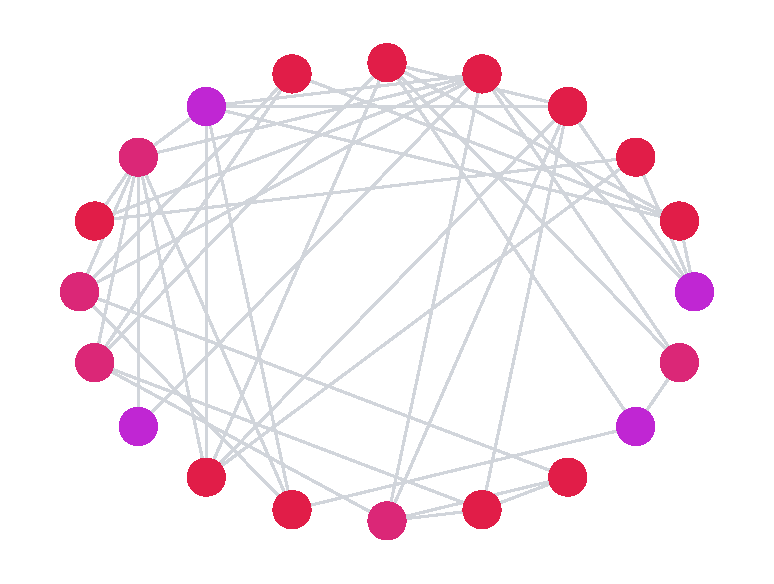
\includegraphics[width=0.8\linewidth]{snapshot}
  \caption{An example of a social network graph.}
\end{figure}

\medskip

\noindent To simulate the opinion diffusion, each simulation holds an internal discrete "clock". This clock is incremented by one after each \emph{round}. A round is over when all nodes decide whether to adopt an opinion of one of their neighbors or retain their current opinion. Each simulation run can be configured with the following parameters:

\begin{itemize}
	\setlength\itemsep{0.2em}

	\item \verb|opinions|: A key-value record, where the key is an identifier of an opinion, and the value is the \emph{probability this opinion will be retained} (unchanged) in the next round.
	\item \verb|colors|: A list of HEX color codes used in graph visualization. Each opinion will use one of these colors in the exported graphs. The length of this list has to be equal to or greater than the number of available opinions.
	\item \verb|runs|: An integer value specifying how many simulations run the program should run. Each simulation run will start with the same graph representation and the same initial node states.
	\item \verb|freeze_length|: An integer value specifying the minimum number of rounds a node will keep a newly adopted state.
	\item \verb|finish_time|: A number of rounds in one simulation run.
\end{itemize}

\section{Algorithm and complexity}
\label{Section:Alg}

The algorithm controlling the flow of the simulation is a linear loop of \verb|finish_time| rounds. In each round, every social network node randomly selects a neighboring node. Then, based on the retention probability of the neighboring node's opinion, it chooses whether to adopt the new opinion or not. 

\begin{figure}[H]
  \begin{minipage}[b]{0.5\linewidth}
    \centering
    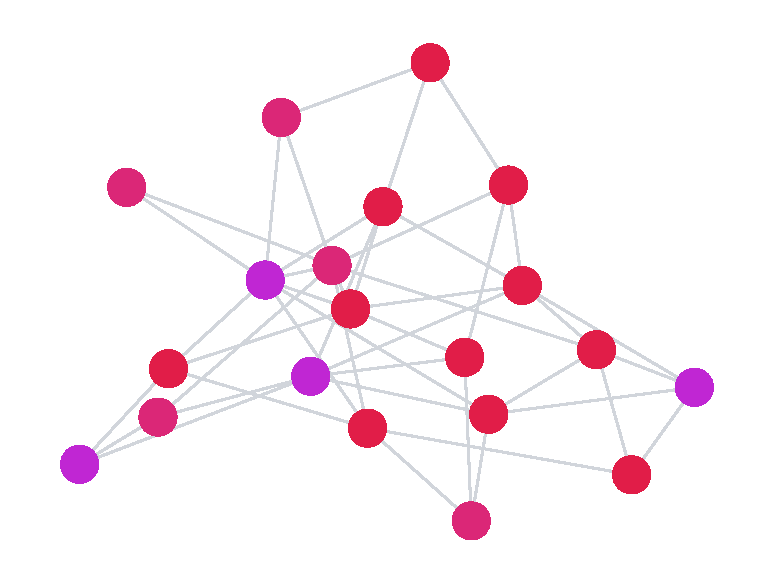
\includegraphics[width=\linewidth]{results/01/run-1/snapshot-0}
    \caption{A social network with two opinions.}
  \end{minipage}%%
  \begin{minipage}[b]{0.5\linewidth}
    \centering
    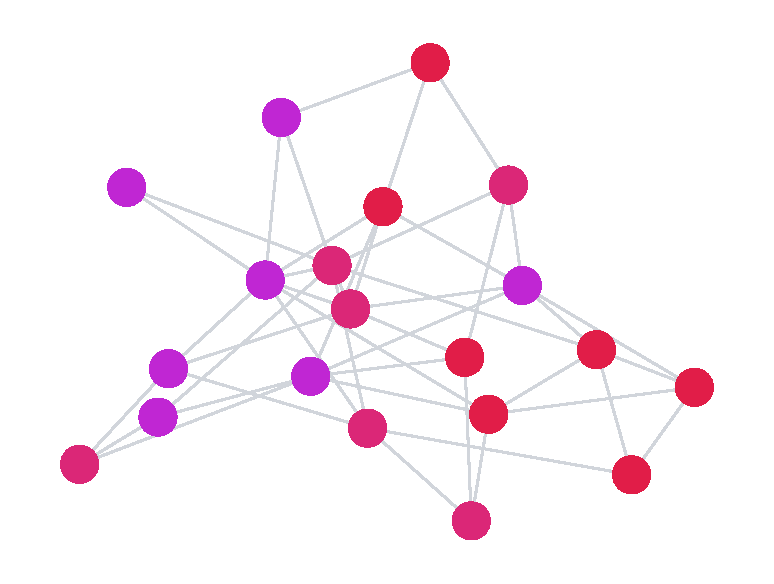
\includegraphics[width=\linewidth]{results/01/run-1/snapshot-5}
    \caption{The same social network after 5 rounds.}
  \end{minipage}
\end{figure}

\medskip

\noindent All opinion changes are only committed (written) at the end of the round to simulate these events simultaneously. Because of this, the algorithm could be potentially run in parallel to improve performance.

\section{Finding important nodes}
\label{Section:Finding}

As the assignment dictates, the neighbors for opinion adoption are selected by a random tournament. Because of this, each individual node of the network has exactly the same importance as other nodes.

\medskip

\noindent One option is to find clusters of nodes with the same opinion. In these clusters, the outer nodes have higher importance than the inner nodes, as only the outer nodes can possibly change their opinion in the next round. Increasing or reducing the opinion adoption of these nodes could have an effect on opinion diffusion.

\begin{figure}[H]
  \centering
  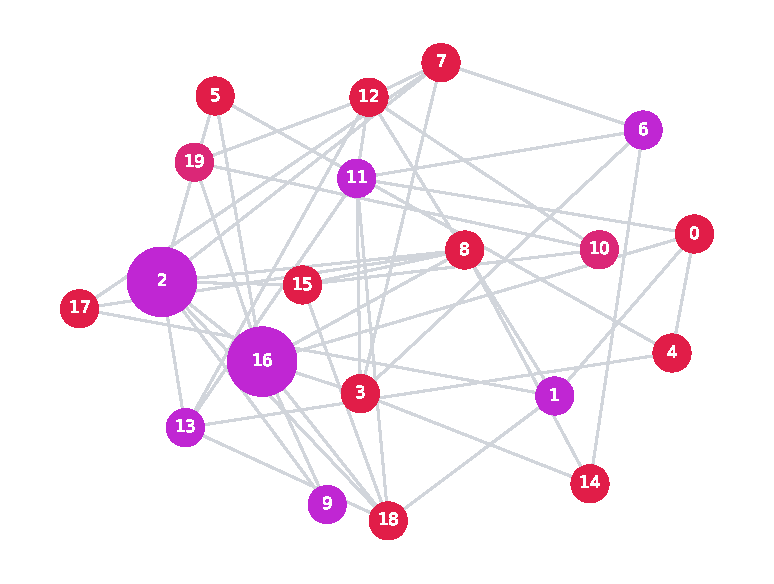
\includegraphics[width=\linewidth]{snapshot-labeled}
  \caption{An example of a social network graph.}
\end{figure}

\noindent Another option is to identify a node (or a set of nodes) that interconnects clusters of nodes in the network. It is possible to use the \emph{betweenness centrality} measure to identify these nodes as the value is higher for the nodes in question. The figure 4 shows a social network graph where the two nodes with the highest betweenness centrality (2, 16) are highlighted. Blocking the opinion adoption of one or both of these nodes would severely affect opinion diffusion as these nodes interconnect multiple clusters of nodes.

\section{Experiments}
\label{Section:Experiments}

Each experiment has an assigned number that corresponds to the dataset used in this experiment. For example, the data used for Experiment 01 can be found in the folder \verb|data/01|. All datasets have been generated using the \verb|gaussian_random_partition_graph| method. Parameters of the generation can be found in the \verb|README.md| file included in each dataset.

\pagebreak

\subsection*{Experiment 01: 20 nodes, 3 opinions}

The experiment features 20 nodes and 3 opinions ("A", "B", "C") with the following probabilities of opinion retention \verb|(A=0.4, B=0.2, C=0.2)|.

\medskip

\noindent The opinion freeze length (\verb|freeze_length|) was set to 4 rounds. The number of simulation runs (\verb|runs|) was set to 4, with each run finishing (\verb|finish_time|) after 50 rounds.

\begin{figure}[ht] 
  \label{ fig7} 
  \begin{minipage}[b]{0.5\linewidth}
    \centering
    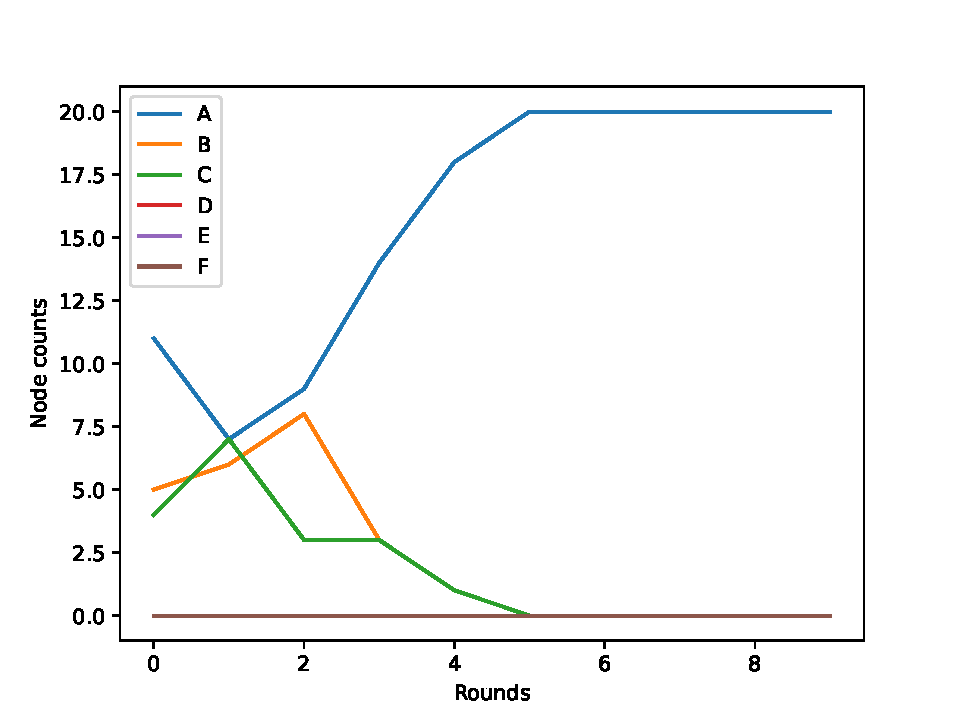
\includegraphics[width=0.9\linewidth]{results/01/run-1/distribution} 
    \caption{Node distribution of the first run.} 
  \end{minipage}%%
  \begin{minipage}[b]{0.5\linewidth}
    \centering
    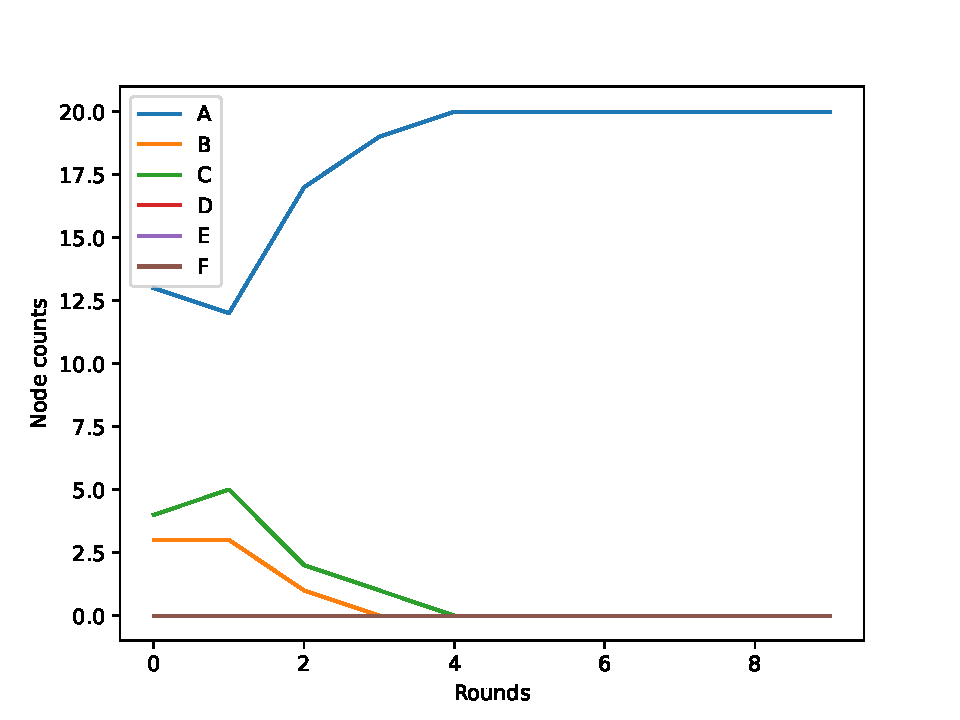
\includegraphics[width=0.9\linewidth]{results/01/run-2/distribution} 
    \caption{Node distribution of the second run.}
  \end{minipage} 
  \begin{minipage}[b]{0.5\linewidth}
    \centering
    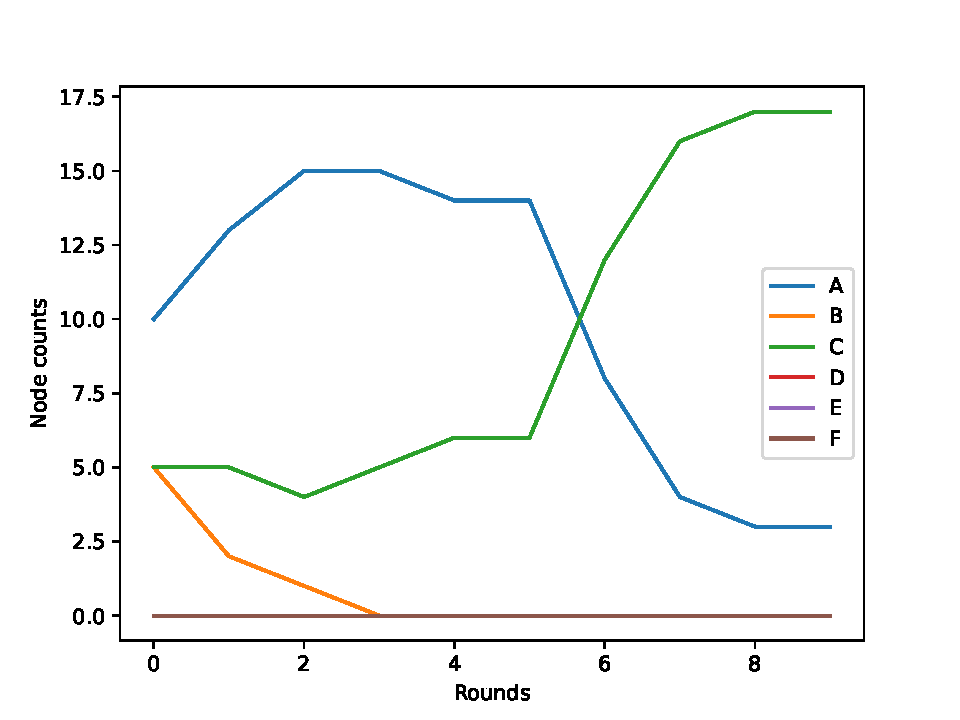
\includegraphics[width=0.9\linewidth]{results/01/run-3/distribution} 
	\caption{Node distribution of the third run.}
  \end{minipage}%% 
  \begin{minipage}[b]{0.5\linewidth}
    \centering
    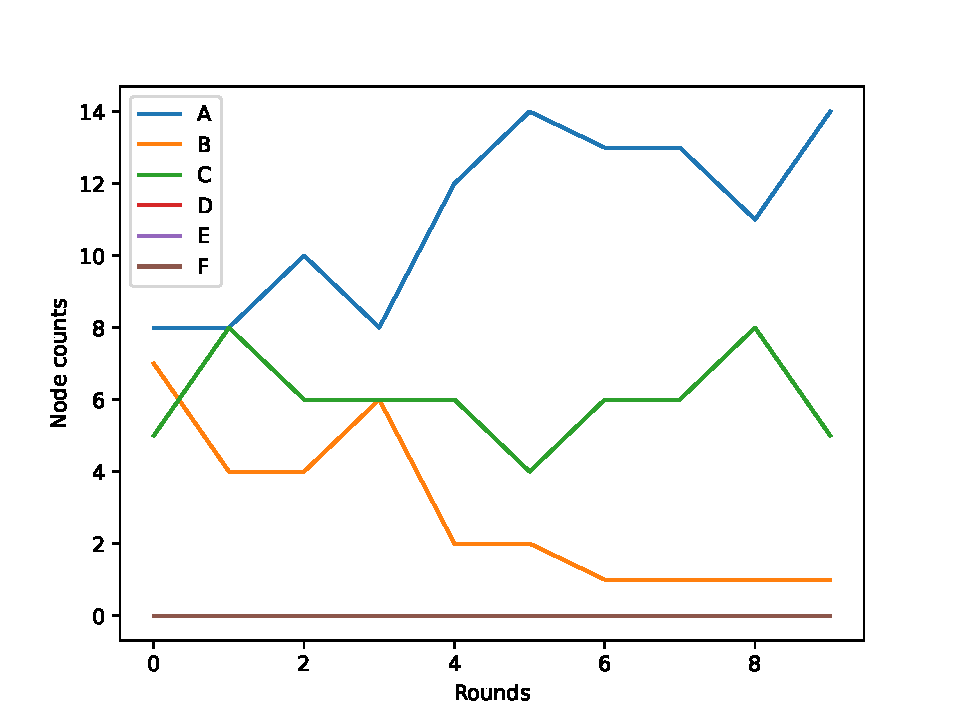
\includegraphics[width=0.9\linewidth]{results/01/run-4/distribution} 
	\caption{Node distribution of the fourth run.}
  \end{minipage} 
\end{figure}

\begin{figure}[h]
	\centering
	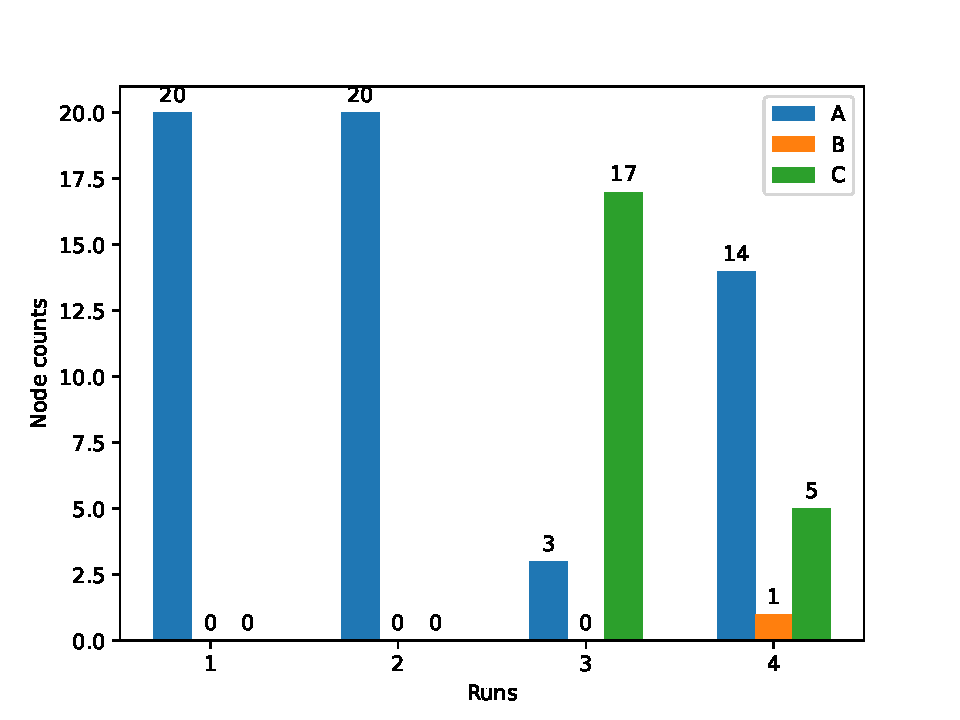
\includegraphics[width=0.5\linewidth]{results/01/distribution} 
	\caption{Node distribution in the final step of each run.}
\end{figure}

\pagebreak

\subsection*{Experiment 02: 50 nodes, 4 opinions}

The experiment features 50 nodes and 4 opinions ("A", "B", "C", "D") with the following probabilities of opinion retention \verb|(A=0.4, B=0.2, C=0.2, D=0.4)|.

\medskip

\noindent The opinion freeze length (\verb|freeze_length|) was set to 4 rounds. The number of simulation runs (\verb|runs|) was set to 4, with each run finishing (\verb|finish_time|) after 80 rounds.

\begin{figure}[ht] 
  \label{ fig7} 
  \begin{minipage}[b]{0.5\linewidth}
    \centering
    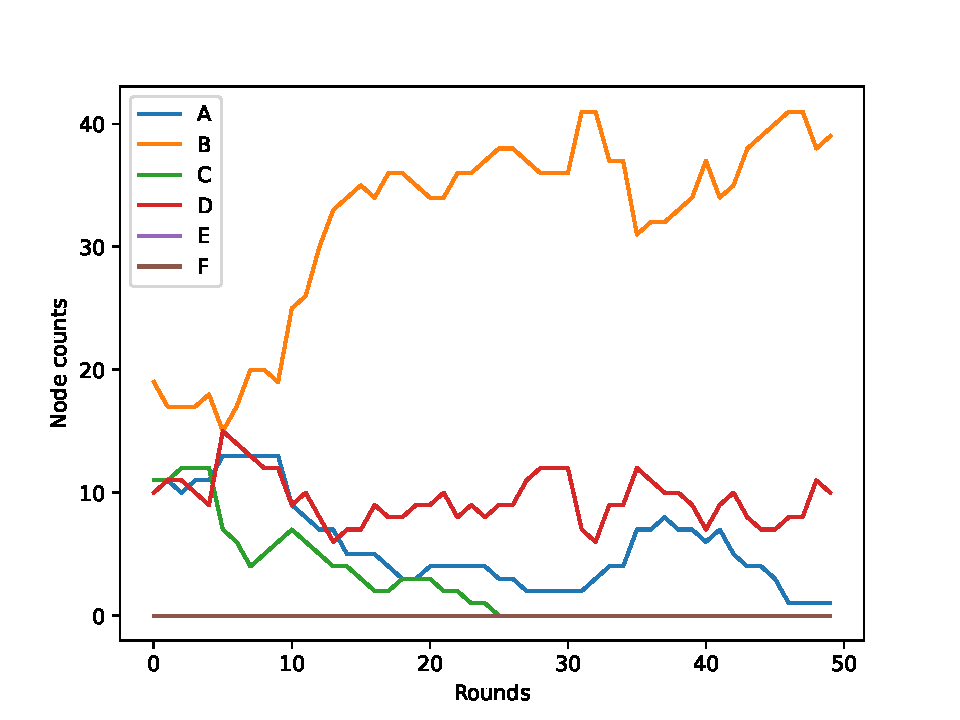
\includegraphics[width=0.9\linewidth]{results/02/run-1/distribution} 
    \caption{Node distribution of the first run.} 
  \end{minipage}%%
  \begin{minipage}[b]{0.5\linewidth}
    \centering
    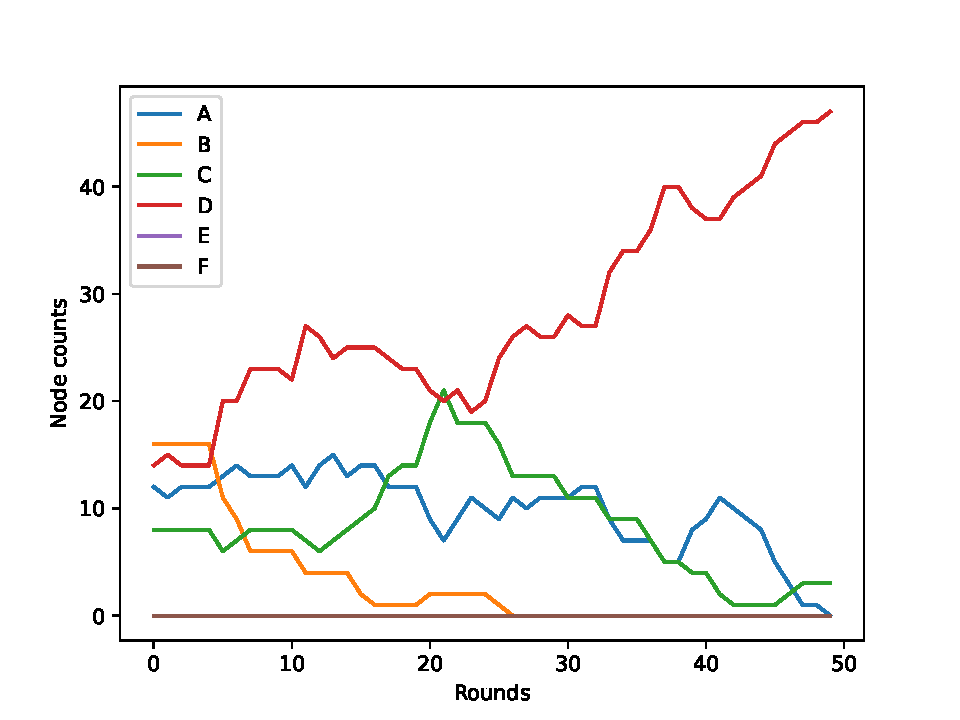
\includegraphics[width=0.9\linewidth]{results/02/run-2/distribution} 
    \caption{Node distribution of the second run.}
  \end{minipage} 
  \begin{minipage}[b]{0.5\linewidth}
    \centering
    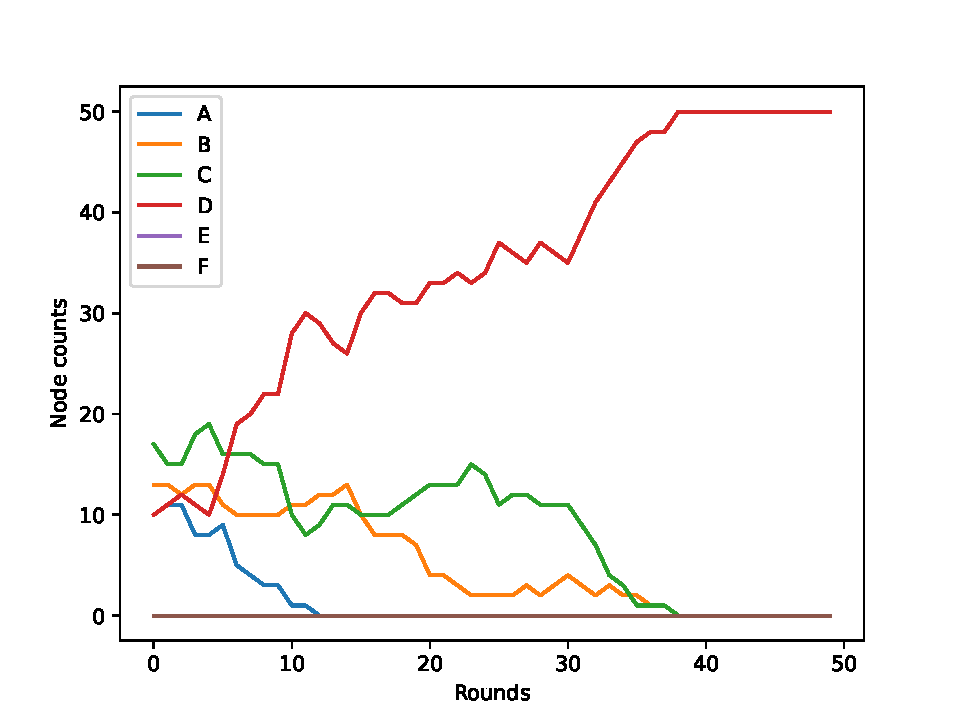
\includegraphics[width=0.9\linewidth]{results/02/run-3/distribution} 
	\caption{Node distribution of the third run.}
  \end{minipage}%% 
  \begin{minipage}[b]{0.5\linewidth}
    \centering
    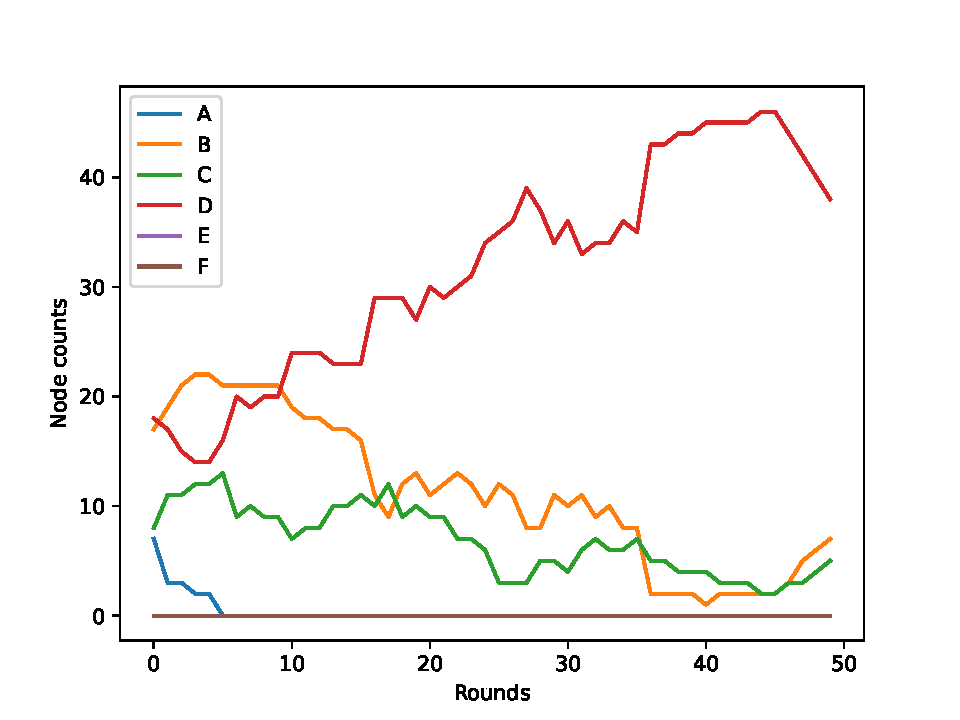
\includegraphics[width=0.9\linewidth]{results/02/run-4/distribution} 
	\caption{Node distribution of the fourth run.}
  \end{minipage} 
\end{figure}

\begin{figure}[h]
	\centering
	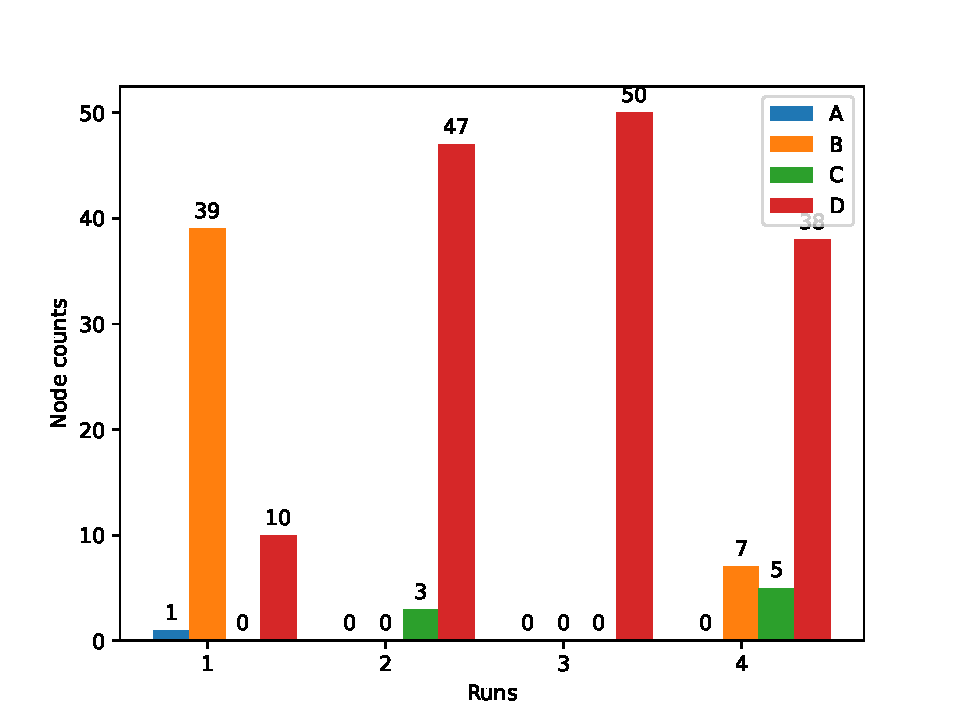
\includegraphics[width=0.5\linewidth]{results/02/distribution} 
	\caption{Node distribution in the final step of each run.}
\end{figure}

\pagebreak

\subsection*{Experiment 03: 200 nodes, 5 opinions}

The experiment features 200 nodes and 5 opinions ("A", "B", "C", "D", "E") with the following probabilities of opinion retention \verb|(A=0.4, B=0.2, C=0.2, D=0.4, E=0.6)|.

\medskip

\noindent The opinion freeze length (\verb|freeze_length|) was set to 6 rounds. The number of simulation runs (\verb|runs|) was set to 4, with each run finishing (\verb|finish_time|) after 200 rounds.

\begin{figure}[ht] 
  \label{ fig7} 
  \begin{minipage}[b]{0.5\linewidth}
    \centering
    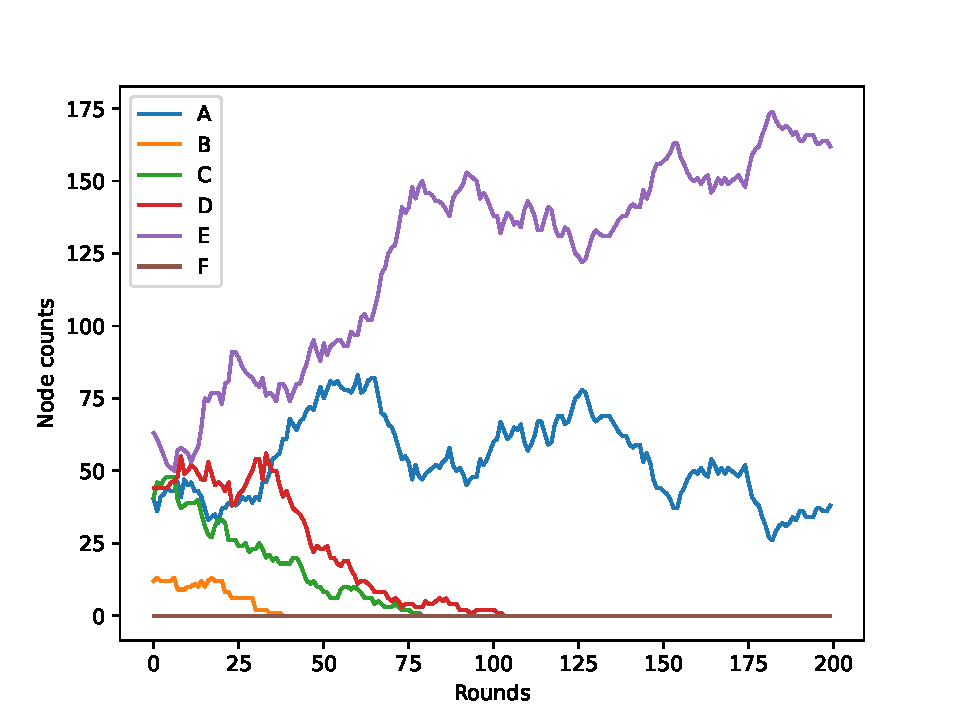
\includegraphics[width=0.9\linewidth]{results/03/run-1/distribution} 
    \caption{Node distribution of the first run.} 
  \end{minipage}%%
  \begin{minipage}[b]{0.5\linewidth}
    \centering
    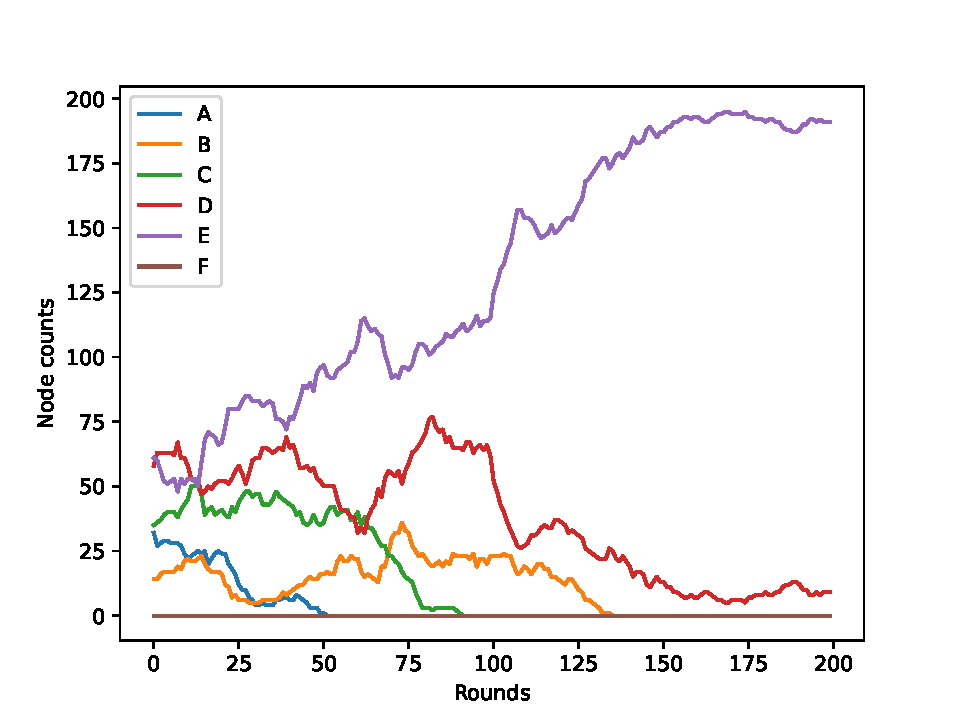
\includegraphics[width=0.9\linewidth]{results/03/run-2/distribution} 
    \caption{Node distribution of the second run.}
  \end{minipage} 
  \begin{minipage}[b]{0.5\linewidth}
    \centering
    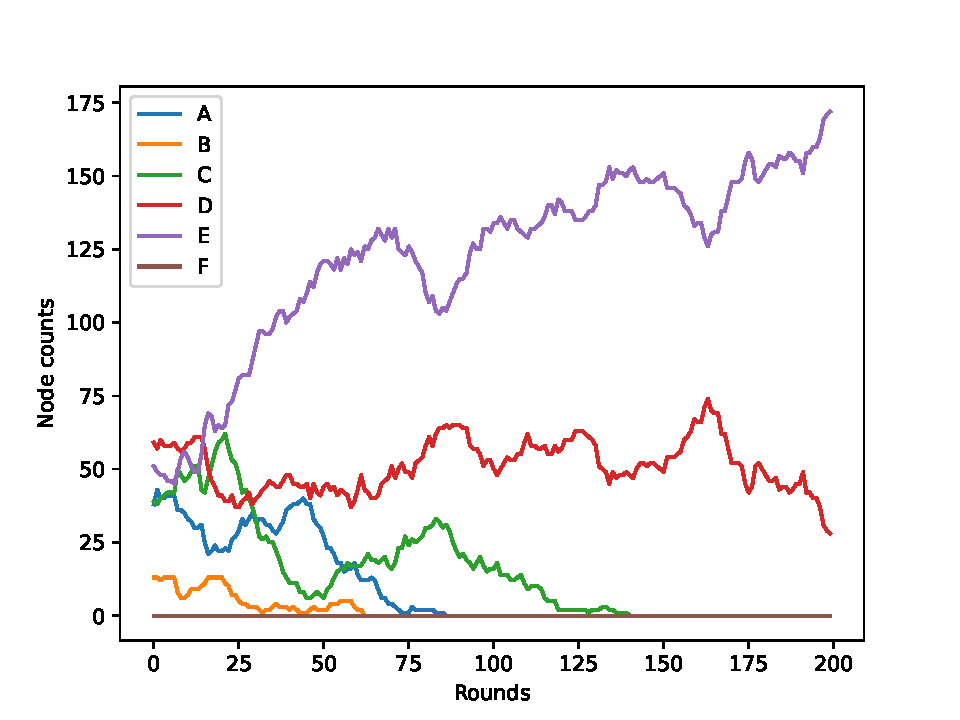
\includegraphics[width=0.9\linewidth]{results/03/run-3/distribution} 
	\caption{Node distribution of the third run.}
  \end{minipage}%% 
  \begin{minipage}[b]{0.5\linewidth}
    \centering
    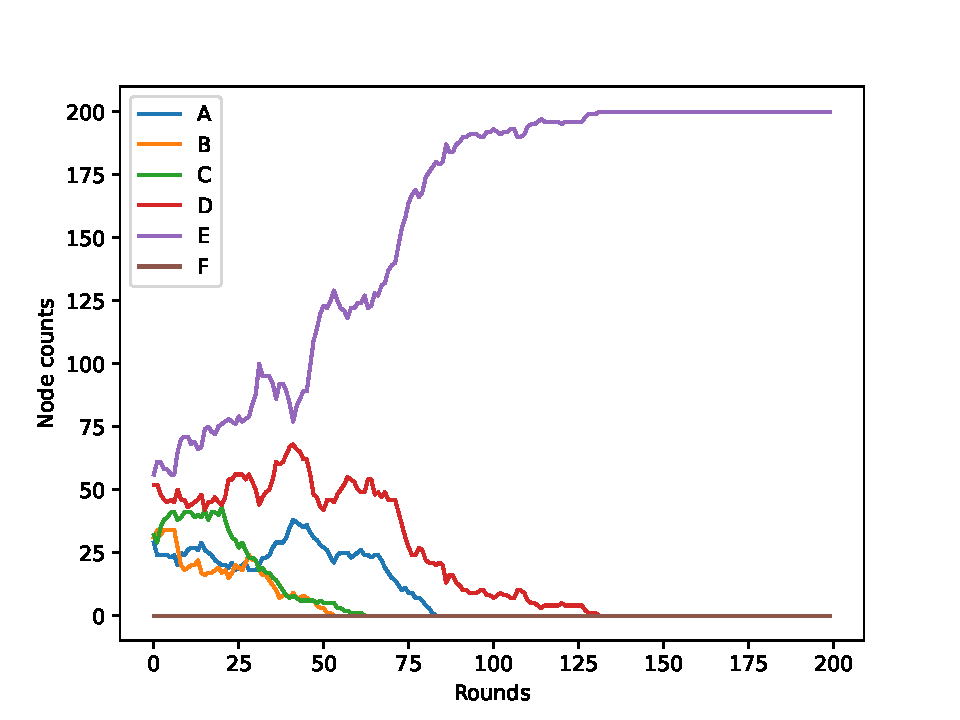
\includegraphics[width=0.9\linewidth]{results/03/run-4/distribution} 
	\caption{Node distribution of the fourth run.}
  \end{minipage} 
\end{figure}

\begin{figure}[h]
	\centering
	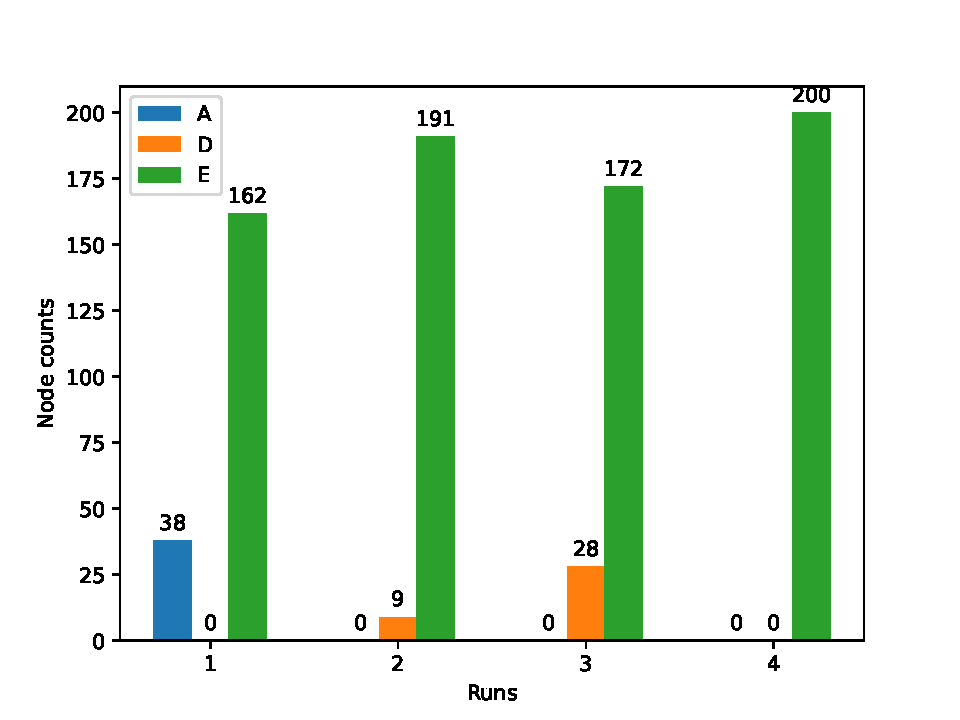
\includegraphics[width=0.5\linewidth]{results/03/distribution} 
	\caption{Node distribution in the final step of each run.}
\end{figure}

\pagebreak

\subsection*{Experiment 04: 1000 nodes, 6 opinions}

The experiment features 1000 nodes and 6 opinions ("A", "B", "C", "D", "E", "F") with the following probabilities of opinion retention \verb|(A=0.4, B=0.2, C=0.2, D=0.4, E=0.6, F=0.4)|.

\medskip

\noindent The opinion freeze length (\verb|freeze_length|) was set to 10 rounds. The number of simulation runs (\verb|runs|) was set to 4, with each run finishing (\verb|finish_time|) after 400 rounds.

\begin{figure}[ht] 
  \label{ fig7}
  \begin{minipage}[b]{0.5\linewidth}
    \centering
    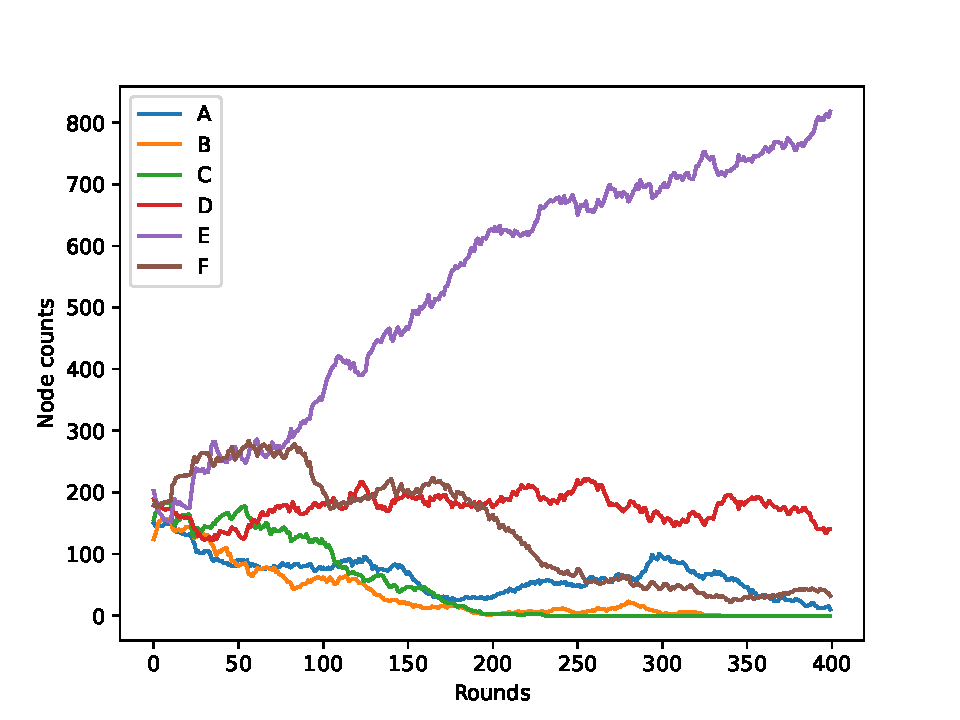
\includegraphics[width=0.9\linewidth]{results/04/run-1/distribution} 
    \caption{Node distribution of the first run.} 
  \end{minipage}%%
  \begin{minipage}[b]{0.5\linewidth}
    \centering
    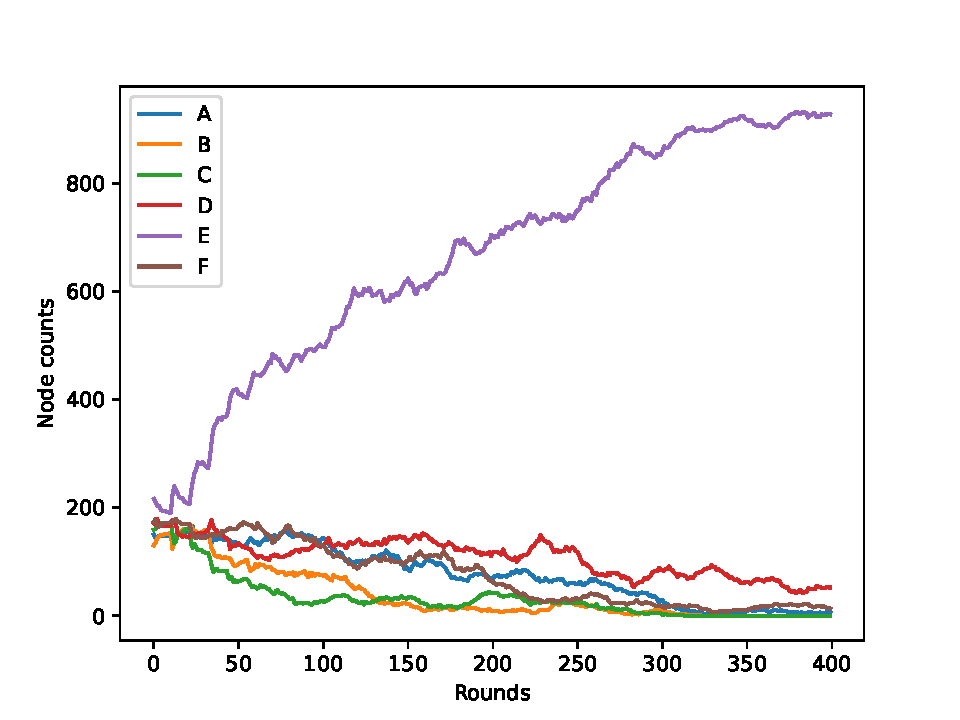
\includegraphics[width=0.9\linewidth]{results/04/run-2/distribution} 
    \caption{Node distribution of the second run.}
  \end{minipage} 
  \begin{minipage}[b]{0.5\linewidth}
    \centering
    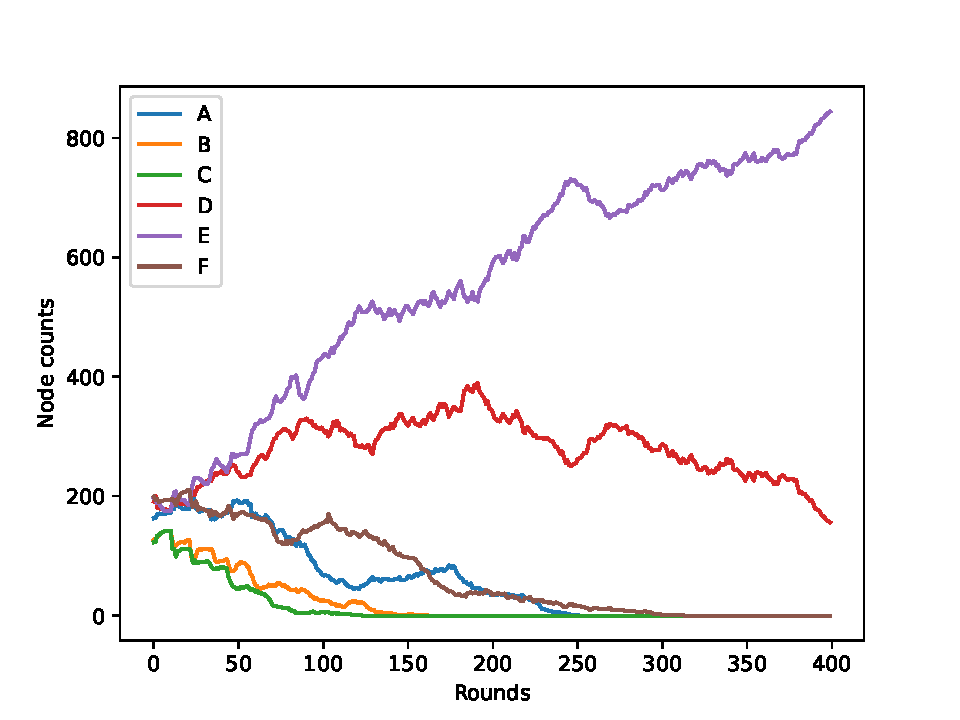
\includegraphics[width=0.9\linewidth]{results/04/run-3/distribution} 
	\caption{Node distribution of the third run.}
  \end{minipage}%% 
  \begin{minipage}[b]{0.5\linewidth}
    \centering
    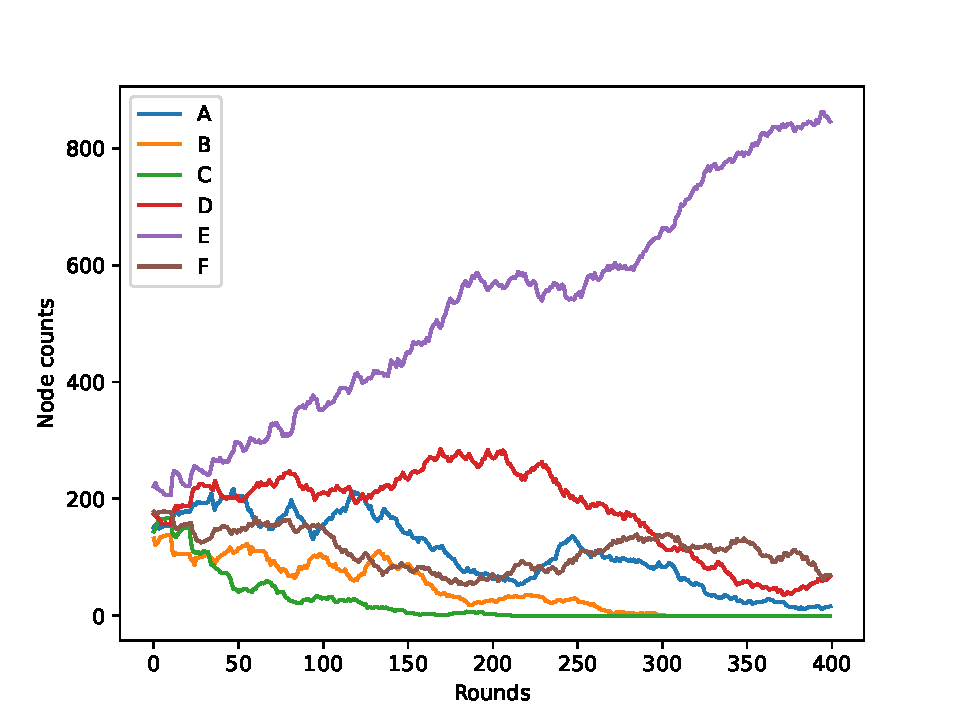
\includegraphics[width=0.9\linewidth]{results/04/run-4/distribution} 
	\caption{Node distribution of the fourth run.}
  \end{minipage}
\end{figure}

\begin{figure}[h]
	\centering
	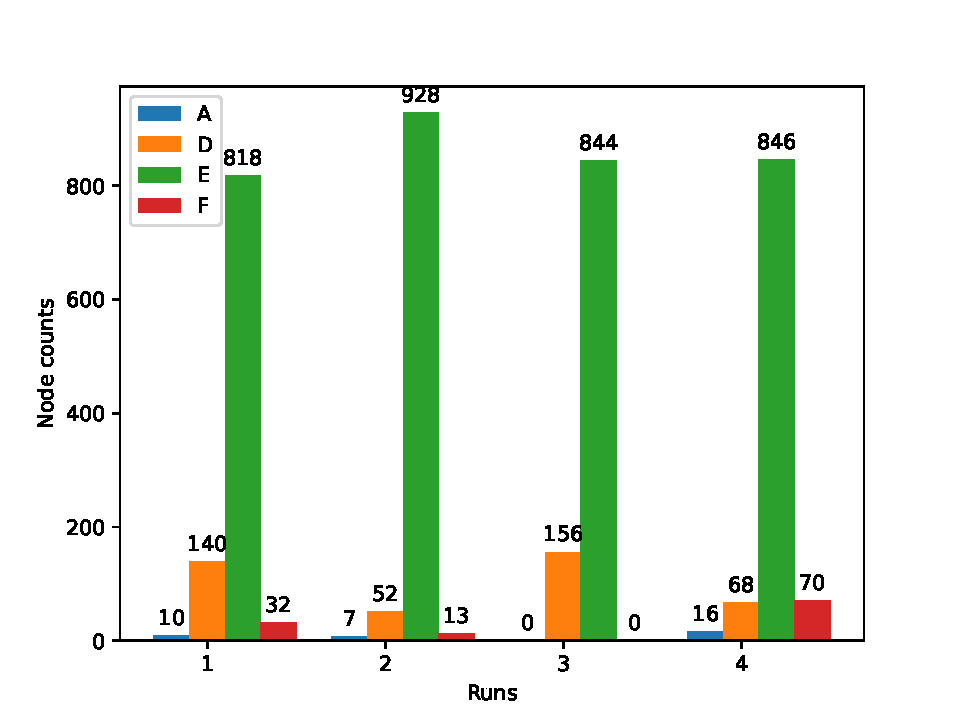
\includegraphics[width=0.5\linewidth]{results/04/distribution} 
	\caption{Node distribution in the final step of each run.}
\end{figure}

\end{document}